% Options for packages loaded elsewhere
% Options for packages loaded elsewhere
\PassOptionsToPackage{unicode}{hyperref}
\PassOptionsToPackage{hyphens}{url}
\PassOptionsToPackage{dvipsnames,svgnames,x11names}{xcolor}
%
\documentclass[
]{ergoclass}
\usepackage{xcolor}
\usepackage{amsmath,amssymb}
\setcounter{secnumdepth}{5}
\usepackage{iftex}
\ifPDFTeX
  \usepackage[T1]{fontenc}
  \usepackage[utf8]{inputenc}
  \usepackage{textcomp} % provide euro and other symbols
\else % if luatex or xetex
  \usepackage{unicode-math} % this also loads fontspec
  \defaultfontfeatures{Scale=MatchLowercase}
  \defaultfontfeatures[\rmfamily]{Ligatures=TeX,Scale=1}
\fi
\usepackage[]{mathpazo}
\ifPDFTeX\else
  % xetex/luatex font selection
\fi
% Use upquote if available, for straight quotes in verbatim environments
\IfFileExists{upquote.sty}{\usepackage{upquote}}{}
\IfFileExists{microtype.sty}{% use microtype if available
  \usepackage[]{microtype}
  \UseMicrotypeSet[protrusion]{basicmath} % disable protrusion for tt fonts
}{}
\makeatletter
\@ifundefined{KOMAClassName}{% if non-KOMA class
  \IfFileExists{parskip.sty}{%
    \usepackage{parskip}
  }{% else
    \setlength{\parindent}{0pt}
    \setlength{\parskip}{6pt plus 2pt minus 1pt}}
}{% if KOMA class
  \KOMAoptions{parskip=half}}
\makeatother
% Make \paragraph and \subparagraph free-standing
\makeatletter
\ifx\paragraph\undefined\else
  \let\oldparagraph\paragraph
  \renewcommand{\paragraph}{
    \@ifstar
      \xxxParagraphStar
      \xxxParagraphNoStar
  }
  \newcommand{\xxxParagraphStar}[1]{\oldparagraph*{#1}\mbox{}}
  \newcommand{\xxxParagraphNoStar}[1]{\oldparagraph{#1}\mbox{}}
\fi
\ifx\subparagraph\undefined\else
  \let\oldsubparagraph\subparagraph
  \renewcommand{\subparagraph}{
    \@ifstar
      \xxxSubParagraphStar
      \xxxSubParagraphNoStar
  }
  \newcommand{\xxxSubParagraphStar}[1]{\oldsubparagraph*{#1}\mbox{}}
  \newcommand{\xxxSubParagraphNoStar}[1]{\oldsubparagraph{#1}\mbox{}}
\fi
\makeatother


\usepackage{longtable,booktabs,array}
\usepackage{calc} % for calculating minipage widths
% Correct order of tables after \paragraph or \subparagraph
\usepackage{etoolbox}
\makeatletter
\patchcmd\longtable{\par}{\if@noskipsec\mbox{}\fi\par}{}{}
\makeatother
% Allow footnotes in longtable head/foot
\IfFileExists{footnotehyper.sty}{\usepackage{footnotehyper}}{\usepackage{footnote}}
\makesavenoteenv{longtable}
\usepackage{graphicx}
\makeatletter
\newsavebox\pandoc@box
\newcommand*\pandocbounded[1]{% scales image to fit in text height/width
  \sbox\pandoc@box{#1}%
  \Gscale@div\@tempa{\textheight}{\dimexpr\ht\pandoc@box+\dp\pandoc@box\relax}%
  \Gscale@div\@tempb{\linewidth}{\wd\pandoc@box}%
  \ifdim\@tempb\p@<\@tempa\p@\let\@tempa\@tempb\fi% select the smaller of both
  \ifdim\@tempa\p@<\p@\scalebox{\@tempa}{\usebox\pandoc@box}%
  \else\usebox{\pandoc@box}%
  \fi%
}
% Set default figure placement to htbp
\def\fps@figure{htbp}
\makeatother





\setlength{\emergencystretch}{3em} % prevent overfull lines

\providecommand{\tightlist}{%
  \setlength{\itemsep}{0pt}\setlength{\parskip}{0pt}}



 
\usepackage[]{natbib}
\bibliographystyle{apalike}


% Additional packages can be loaded here if needed
% The ergoclass already loads most necessary packages

% Uncomment if you need these:
% \usepackage{booktabs}
% \usepackage{longtable}
\makeatletter
\@ifpackageloaded{float}{}{\usepackage{float}}
\floatstyle{plain}
\@ifundefined{c@chapter}{\newfloat{apptbl}{h}{loapptbl}}{\newfloat{apptbl}{h}{loapptbl}[chapter]}
\floatname{apptbl}{Table A}
\newcommand*\quartoapptblref[1]{Table \hyperref[#1]{A\ref{#1}}}
\@ifpackageloaded{caption}{}{\usepackage{caption}}
\DeclareCaptionLabelFormat{quartoapptblreflabelformat}{#1#2}
\captionsetup[apptbl]{labelformat=quartoapptblreflabelformat}
\newcommand*\listofapptbls{\listof{apptbl}{List of Table As}}
\makeatother
\makeatletter
\@ifpackageloaded{caption}{}{\usepackage{caption}}
\AtBeginDocument{%
\ifdefined\contentsname
  \renewcommand*\contentsname{Table of contents}
\else
  \newcommand\contentsname{Table of contents}
\fi
\ifdefined\listfigurename
  \renewcommand*\listfigurename{List of Figures}
\else
  \newcommand\listfigurename{List of Figures}
\fi
\ifdefined\listtablename
  \renewcommand*\listtablename{List of Tables}
\else
  \newcommand\listtablename{List of Tables}
\fi
\ifdefined\figurename
  \renewcommand*\figurename{Figure}
\else
  \newcommand\figurename{Figure}
\fi
\ifdefined\tablename
  \renewcommand*\tablename{Table}
\else
  \newcommand\tablename{Table}
\fi
}
\@ifpackageloaded{float}{}{\usepackage{float}}
\floatstyle{ruled}
\@ifundefined{c@chapter}{\newfloat{codelisting}{h}{lop}}{\newfloat{codelisting}{h}{lop}[chapter]}
\floatname{codelisting}{Listing}
\newcommand*\listoflistings{\listof{codelisting}{List of Listings}}
\makeatother
\makeatletter
\makeatother
\makeatletter
\@ifpackageloaded{caption}{}{\usepackage{caption}}
\@ifpackageloaded{subcaption}{}{\usepackage{subcaption}}
\makeatother
\usepackage{bookmark}
\IfFileExists{xurl.sty}{\usepackage{xurl}}{} % add URL line breaks if available
\urlstyle{same}
\hypersetup{
  pdftitle={When are Philosophy Articles Cited?},
  pdfauthor={Anon},
  colorlinks=true,
  linkcolor={blue},
  filecolor={Maroon},
  citecolor={Blue},
  urlcolor={Blue},
  pdfcreator={LaTeX via pandoc}}


\title{When are Philosophy Articles Cited?}

\author{Anon}
\affiliation{Anon Institution}
\contact{anon@institution.edu}


\textofabstract{%
It's natural to believe that philosophy citations are typically to long
ago pieces. We're still talking about philosophers from millenia ago.
More strikingly, we're still talking about papers from half a century
ago not as historical papers, but as part of the contemporary debate.
But a systematic look at the citation data shows that these cases are
outliers. Most citations are to recently published works. Surprisingly,
this is less true in recent years than it used to be. The effect of
electronic publishing and communication has been to make citations, on
average, older. After we adjust for the typical age of philosophy
citations, and this changing trend, it turns out that the 2000s were a
particularly influential time in philosophy publishing. Articles
published in that decade are cited more than earlier or later articles,
once we adjust for the typical times articles are cited, and the
changing patterns of citation. This is arguably related to broad changes
in the interests of philosophers, towards social philosophy, and
epistemology.
}%

\articledoi{https://doi.org/TBC}

\volumeissueyear{TBC}{TBC}{2025}%

\setcounter{page}{1}%

\begin{document}
\maketitle

\section{Introduction}\label{sec-introduction}

This paper is about the patterns of citations of philosophy journal
articles in philosophy journals. Obviously philosophy journals cite more
things than philosophy journals, and just as obviously philosophy
journal articles get cited in other places. But looking just at
journal-to-journal citations allows us to get a citation set that is
relatively complete, and hence make some systematic generalisations
about the way articles are cited over time. It turns out some of these
generalisations are surprising.

Before looking at the data, here are two things I believed about
philosophy citations. First, philosophers tend to cite very old papers.
We still regularly teach a number of papers over half a century old in
introductory classes; e.g., \citet{WOSA1969Y444700002},
\citet{WOSA1971Y116900003}, \citet{WOSA1972Z066400001}, and
\citet{10.2307_2025310}. These aren't taught as history papers, but as
early entries into the contemporary philosophical debate. While most
papers aren't cited as much as these papers are, I thought the pattern
that old papers keep being cited extended to their less famous
counterparts. Second, the technological changes of the last quarter
century meant that this practice was being slowly reversed. A series of
technological innovations made it easier to cite newer and newer works.
These innovations included the spread of email, the rise of preprint
archives (e.g., arXiv, SSRN, PhilPapers), and eventually official
preprints in things like EarlyView. So, I thought, citations should be
getting younger, because the delay between publishing and getting widely
known was removed.

Both of these thoughts were wrong.

On the first point, the generalisation I made from those famous papers
was just wrong. Normal papers differ from famous papers not just in how
often they are cited, but in the shape of their citations. The main
evidence I'll use for this is something I'll call the \emph{citation
ratio}. The citation ratio of year \emph{o} in year \emph{n} is the mean
number of citations, in year \emph{n}, of articles published in year
\emph{o}, divided by the mean number of citations, in year \emph{n}, of
articles published in years \emph{n}-10 to \emph{n}-3. (I'll say much
more about why I'm using this measure in what follows.)
Figure~\ref{fig-master-citation-ratio} shows the average citation ratio
for different \emph{ages}, of citations, i.e., the number of years
between \emph{o} and \emph{n}.\footnote{The graph also includes some
  `jitter' to make the different points more easily visible. I've put
  each decade of original publication in a different colour; I'll break
  those out in Figure~\ref{fig-decades-cite-ratio}. The graph starts in
  1975 because the data is much noisier before then, for reasons we'll
  get to below.}

\begin{figure}

\centering{

\pandocbounded{\includegraphics[keepaspectratio]{apc-2025-october-draft_files/figure-pdf/fig-master-citation-ratio-1.pdf}}

}

\caption{\label{fig-master-citation-ratio}Age effects from 1975 onwards
on a single graph, with the overall average shown.}

\end{figure}%

Each dot on that graph is a citation ratio for a particular pair of
years; the line shows the average citation ratio for all pairs with the
same age. The shape is unmistakable; articles get cited much much more
when they are relatively young than when they are older.

The `evidence' I gave for the opposite view in the introductory
paragraph wasn't entirely wrong. If we redo
Figure~\ref{fig-master-citation-ratio} just looking at articles which
have 15 or more citations in philosophy journals, we get
Figure~\ref{fig-ageeffecteverything-high}. (Restricting to these
articles means we look at a small percentage of a articles, but a decent
percentage of the citations.)

\begin{figure}

\centering{

\pandocbounded{\includegraphics[keepaspectratio]{apc-2025-october-draft_files/figure-pdf/fig-ageeffecteverything-high-1.pdf}}

}

\caption{\label{fig-ageeffecteverything-high}A version of
Figure~\ref{fig-master-citation-ratio} just looking at highly cited
articles}

\end{figure}%

The numbers on the y-axis in Figure~\ref{fig-ageeffecteverything-high}
are higher than in Figure~\ref{fig-master-citation-ratio}. That's not
surprising; it just means highly cited articles get cited more
frequently. What is striking is the different shape of the graphs.
Typical philosophy articles, if they get cited at all, get cited soon
after publication and they fade into obscurity. Highly cited articles
keep getting cited decades after their publication.

These results aren't a priori obvious; things could have turned out
otherwise. It could have been that there were a trove of articles which
were ignored after publication and then accrued five to ten citations a
couple of decades later. There are some articles that were very
frequently cited soon after publication but which are now largely
ignored. (This happens most frequently in philosophy of science and in
philosophy of mind, I think for different reasons in the two cases.) But
these cases are outliers. Most of the articles that were influential
soon after publication stay that way.

For the second point, we can simply break up
Figure~\ref{fig-master-citation-ratio} by ten year chunks. In
Figure~\ref{fig-decades-cite-ratio} I've taken the points by from
Figure~\ref{fig-master-citation-ratio}, and grouped them into `decades'.
Because I'm working here with 1975-2024 data, the decades are 1975-1984,
1985-1994 etc. To make it easier to compare decades, I've removed the
last one, where there isn't enough data, and removed all points with an
age over 20.

\begin{figure}

\begin{minipage}{0.50\linewidth}

\centering{

\pandocbounded{\includegraphics[keepaspectratio]{apc-2025-october-draft_files/figure-pdf/fig-decades-cite-ratio-1.pdf}}

}

\subcaption{\label{fig-decades-cite-ratio-1}1975-1984}

\end{minipage}%
%
\begin{minipage}{0.50\linewidth}

\centering{

\pandocbounded{\includegraphics[keepaspectratio]{apc-2025-october-draft_files/figure-pdf/fig-decades-cite-ratio-2.pdf}}

}

\subcaption{\label{fig-decades-cite-ratio-2}1985-1994}

\end{minipage}%
\newline
\begin{minipage}{0.50\linewidth}

\centering{

\pandocbounded{\includegraphics[keepaspectratio]{apc-2025-october-draft_files/figure-pdf/fig-decades-cite-ratio-3.pdf}}

}

\subcaption{\label{fig-decades-cite-ratio-3}1995-2004}

\end{minipage}%
%
\begin{minipage}{0.50\linewidth}

\centering{

\pandocbounded{\includegraphics[keepaspectratio]{apc-2025-october-draft_files/figure-pdf/fig-decades-cite-ratio-4.pdf}}

}

\subcaption{\label{fig-decades-cite-ratio-4}2005-2014}

\end{minipage}%

\caption{\label{fig-decades-cite-ratio}Citation ratio for different
decades}

\end{figure}%

There are three general trends across these graphs, especially after the
second graph.

\begin{enumerate}
\def\labelenumi{\arabic{enumi}.}
\tightlist
\item
  The peaks are getting later. In the first two graphs, the line is
  clearly heading down by age 5; in the last one it is barely off the
  peak at that time.
\item
  The peaks are getting lower. In the last graph we barely see it cross
  1.
\item
  The declines are much, much flatter. If you look around age 15 in the
  four graphs, you see the values rise steadily over time.
\end{enumerate}

What all this means is that citations are getting older. While it's
still true that articles from a year are (collectively) cited a more
often from ages 2-5 than from ages 12-15, the difference between those
two rates has fallen remarkably. The effect of technology on citations
has been the complete opposite of what I expected.

The rest of this paper has two aims.

First, I'm going to set out the methodology behind these graphs, go over
the choices I made in building them, and argue that these were at least
defensible choices. The intended conclusion is that these graphs really
show what I say they do, that traditionally citations were mostly to
very recent articles, but they are now more frequently to older
articles.

Second, I'm going to look citations from various years, after adjusting
for these typical citation rates, and see which years have been more
influential in the later literature. I suspect readers will not be
surprised that the early 1970s stand out as being particularly
influential. What might be more surprising is that the next most
influential period, in terms of how often articles from then are cited
compared to the overall trends, is the 2000s. There are a few possible
reasons for this, but I suspect the main one is the rising importance at
that time of epistemology. (This is something Eugenio
\citet{Petrovich2024} also found using a somewhat different data set.)
More generally, looking at citations from different periods, and
especially looking at which articles make up those citations, is a
useful guide to the history of those periods. Most work on the history
of analytic philosophy doesn't get beyond the early 1970s; this is an
early attempt to quantify what happens in the years after the changes
brought about by Kripke, Lewis, Rawls and others in those years.

\section{Age of Citations}\label{sec-age-of-citations}

\subsection{Methodology}\label{sec-methodology}

The data for this study comes from Web of Science (hereafter, WoS). In
this section I'll go over which data I chose to use, and how I patched
it together.

The bulk of the data comes from the XML files that WoS makes available
to subscribing institutions. Until recently, that included my own, so
that's where most of the data through 2021 comes from. That subscription
has not been renewed, so the data since 2021 comes from the WoS
API.\footnote{This is also via a susbcription through my institution;
  the XML is more expensive.}

The XML file is rather large. After de-compression it's over a terabyte.
To make it manageable, I filtered down to \emph{articles} (as opposed to
discussion notes, book reviews, editorial matters, and so on), and whose
category was either Philosophy or History \& Philosophy of Science. I
then selected by hand the hundred journals with the most inbound
citations (among articles in these categories) which were (a) primarily
English language, (b) not primarily history of science and (c) broadly
`analytic' rather than `continental'. These were somewhat subjective
choices, but the result was a reasonable collection of the journals
which are most important for telling the story of a certain kind of
philosophy over the last several decades.

The list of journals being used, as well as some basic statistical
information about them, is in Section~\ref{sec-statistics}. Once I had
those journals, I included all articles (and notes/reviews over 15
pages) from them. I did not restrict the study to pieces that were
labelled as Philosophy or History \& Philosophy of Science. For
interdisciplinary journals, especially \emph{Mind and Language}, those
labels seemed very unreliable on a paper-by-paper basis, and I preferred
to have a full picture of each journal I was using.

The data from the XML was supplemented in two ways. First, WoS does not
index \emph{The Journal of Philosophy} between 1971 and 1974. It is
missing a few other journals in 1974 in particular, but this gap was the
longest and most important, and I thought I needed to fix it. Between
1971 and 1974 the Journal published groundbreaking articles by Harry
\citet{Frankfurt1971}, George \citet{Boolos1971}, Paul
\citet{Benacerraf1973}, Jaegwon \citet{Kim1973}, Michael
\citet{Friedman1974}, Isaac \citet{Levi1974}, and David Lewis
\citetext{\citeyear{Lewis1971cen}; \citeyear{Lewis1973ben}}. Leaving all
of those papers out seemed like it undermined the story. So I used JSTOR
to find a full list of articles (as opposed to notes or book reviews) in
\emph{Journal of Philosophy} in those years, and then looked through the
citations in articles in Table~\ref{tbl-list-of-journals} to see which
citations were to one of those articles. This did mean I was using a
different classification of publications into articles and non-articles,
and there are some odd choices.\footnote{Notably, the JSTOR list seemed
  to exclude the symposium centered around Kenneth Arrow's ``Some
  Ordinalist-Utilitarian Notes on Rawls's Theory of Justice''; I'm not
  sure why that was.} And it meant I had to do a fair bit of data
cleaning just to track down references to those four years.\footnote{A
  non-trivial chunk of the cleaning was sorting through the many and
  varied ways that philosophers have spelled Brian O'Shaughnessy's name
  over the years.} While I've strived to make the data as consistent as
possible with the other years, it's possible that I haven't succeeded,
and some discontinuities around the early 1970s are due to this
discontinuity in how the data was acquired.

The tables in Section~\ref{sec-introduction} start in 1975 in part
because I'm concerned about the consistency of the data that had to be
complied in two different ways, but largely because WoS only starts
indexing \emph{Analysis} in 1975. Without \emph{Analysis}, and
especially without the papers on the analysis of knowledge and on
inferentialism, you don't get a particularly complete picture of how
citations work in those years. I've included 1956-1974 in some of the
studies below, but the data presented there is much less complete, and
hence they aren't as useful for figuring out larger trends.

The other way I supplemented the XML relates to the fact that the XML I
have only goes through mid-2022. Using the WoS website, I downloaded all
the articles in, and citations in, articles in these 100 journals from
2021-2024. I processed these using the bibliometrix package
(\citet{bibliometrix}). I used the 2021 data to check that this method
yielded roughly the same results as the XML. The differences were not
great - well under 1\% for the number of articles, and a little over 1\%
for the number of citations. So it's not a perfect match, but it's
fairly close. The data used in this study for 2022-2024 comes from the
WoS website via bibliometrix.

\subsection{Journal to Journal}\label{sec-journal-to-journal}

As noted earlier, this study is restricted to a particular kind of
citation: when a philosophy journal article is cited in another
philosophy journal article. That obviously leaves out a lot. The
restriction to journal articles means we exclude edited volumes, theses,
conference programs, and, above all, books. The restriction to
philosophy means that we exclude citations in journals in adjacent
fields.

The reason for these restrictions is threefold.

First, the journal-to-journal data is so much cleaner than any other
data. When WoS records a citation of an article it indexes by an article
it indexes, the citation record includes the WoS ID number for the cited
journal article. That means that we don't have to clean up cases where
the citing author got any details of the cited article wrong. It's very
common for authors to cite incorrect page numbers for an article. It's
less common, but still sufficiently frequent that one has to check it,
for authors to cite incorrect titles, author names (especially for hard
to spell names) or even publication years. Cleaning this is a lot of
work. In practice, restricting attention to cases where WoS includes an
ID number for the cited article does not avoid this problem as much as
delegate it to WoS. Otherwise, doing this is a huge amount of work. A
similar study to this one was earlier done by Eugenio
\citet{Petrovich2024}; he looked at all citations in five leading
philosophy journals. It wasn't practical for him to look at more than
five because of how much work it was to clean all those citations. I'm
losing some comprehensiveness compared to his study, but covering twenty
times more journals. This isn't to say that one of the ways of doing
things is right and the other wrong; rather that by looking at slightly
different things, the two studies should complement each other.

Second, looking at journals allows for a kind of comprehensiveness. To
find out how often the average philosophy book from a particular year
was cited, we'd need a database of all the books. Maybe that's possible
via the Library of Congress, but it would be a challenge. To find out
how often the average paper in an edited volume was published, we'd need
a database of all the chapters in edited volumes. I don't know where one
would start looking for such a thing. Journals have the advantage that
they number their issues; you can typically confirm that you have
everything.

Third, dealing with whole journals makes the challenge of demarcating
philosophy from non-philosophy a little more manageable. At the very
least, I can show you what I mean by a philosophy journal; I mean the
journals listed in Table~\ref{tbl-list-of-journals}. If I had to go
through book-by-book, or chapter-by-chapter, making decisions on which
were inside philosophy, it would be a massive task, and it would be
nearly as massive a task for anyone to double check. The key thing here
is that I'm not attempting to quantify philosophy articles published in
journals, but articles published in philosophy journals. The demarcation
problem is still incredibly challenging; for instance, should I have
included \emph{Cognition} in this study? Invariably some arbitrary
boundaries will be drawn. The upside of the way I'm doing things is that
it involves fewer such boundaries, and they are more visible to you the
reader.

In practice there are two major downsides to restricting attention to
philosophy-journal-to-philosophy-journal citations.

With respect to inbound citations, a big difference is that different
kinds of books and journal articles are cited, and these can give you a
very different impression of the field. History of philosophy does not
involve as much publishing in journals, and the articles that are
published cite primary sources, and more recent books, more than other
journal articles. This kind of work offers essentially zero insight into
developments in the history of philosophy. Also, and this will become
important later, often citations to books are to much older works than
citations to articles. \citet{Petrovich2024} notes that through the
1990s, Quine, Wittgenstein and Davidson are amongst the most cited
authors. None of them show up as near the top if you just look at cited
journal articles.

Davidson, in particular, raises another issue about citations to journal
articles. A citation is only recorded as being to a journal article if
the journal is identified in some way, ideally by name though a DOI
reference would also work, in the citing article. In older works,
citations to famous articles often just mention one or other collection
in which they were reprinted. If someone cites ``Actions, Reasons, and
Causes'', but the only bibliographic detail they give is that it's
chapter one in \emph{Essays on Actions and Events}, it won't necessarily
show up as a journal-to-journal citation in WoS. Most articles aren't
reprinted, and these days people cite originals as well as, or instead
of, reprints. So overall this isn't a huge effect. But if one was trying
to find the most cited articles, it's a huge source of error.\footnote{I
  had been planning a study on which articles had the largest declines
  in citations, as a way of measuring changes in philosophical fashion.
  But most of the articles I found had been reprinted so often that this
  effect explained most of what I found. It isn't a big effect overall,
  but if you go looking for outliers, you'll mostly find cases where the
  data is unreliable.}

With respect to outbound citations, the study I'm doing doesn't show how
often journals are cited outside philosophy. It doesn't show how often
they are cited in books either, but that's less of a problem, I believe,
because citations in books and citations in journals have similar
patterns. But citations inside philosophy are a very poor guide to
citations outside philosophy. If you look at
Table~\ref{tbl-list-of-journals}, you'll see that the articles in
\emph{Journal of Medical Ethics} are, collectively, cited very rarely.
This is almost entirely a consequence of my excluding medical journals
where that journal is cited more often. The data in
Table~\ref{tbl-list-of-journals} tells you something. If you wanted
confirmation that `core' philosophy journals don't publish much
bioethics, the citation numbers for \emph{Journal of Medical Ethics} are
evidence for that. But they are not evidence for anything about the
overall impact of the journal; we just aren't looking in the right place
to see that.

\subsection{Age, Period, and Cohort}\label{sec-apc}

To help understand the citation patterns, I'll borrow some terminology
that's common in both sociology and medicine. It's easiest to introduce
this terminology with an example. Imagine that we see, in the historical
record, some interesting patterns among teenagers in the late 1960s, and
we're wondering what could explain the pattern. Two types of pattern
spring immediately to mind, along with ways to test them.

First, the behaviour could be explained by the fact the people involved
are teenagers. If so, it is an \textbf{age effect}. The natural way to
test this is to see if similar patterns show up with teenagers at
different times.

Second, the behaviour could be explained by the fact that it was the
1960s, and lots of striking things happened in the 1960s. If so, it is a
\textbf{period effect}. The natural way to test this is to see if the
same pattern shows up with non-teenagers in the 1960s.

There is an important third kind of explanation. The people involved are
born in the early 1950s, so they are part of the post-war baby boom.
Colloquially, they are boomers. Maybe that could explain the pattern we
see. If so, it is a \textbf{cohort effect}. The natural way to test this
is to see if the same pattern shows up if we look at the same people in
other stages of their life.

It's easy to overlook the importance of cohort effects. Sometimes they
simply look like age effects. \citet{GhitzaEtAl2023} argue that many
hypotheses about age effects on voting, e.g., that older people are more
naturally conservative, are really just cohort effects. \citet{Bump2023}
argues that understanding the distinctive role the boomers in particular
play is crucial for understanding many aspects of modern American life.

There are mathematical reasons that it is hard to tease these effects
apart too. Many statistical techniques for separating out influences
start to fall apart when there are linear correlations between
combinations of variables. In this case there is as tight a correlation
as is possible. By definition, cohort plus age equals period. There are
some things you can do to get around this problem - see
\citet{KeyesEtAl2010} for a useful survey of some of the options, and
see \citet{Rohrer2025} for some recent scepticism about general
solutions to it - but it remains a challenge.

Even conceptually, it is hard to separate out these three effects in
cases where there is evidence that the strength of the effects changes
over time. As I noted at the start, the natural way to test hypotheses
about which effect is strongest involve looking at other times. That
works well when the age effects are constant. When they are not (and
they might not be here), it is harder.

For most of our story, however, it helps just to have these three
effects in mind. Using them, we can summarise the data reasonably
quickly.

\begin{itemize}
\tightlist
\item
  The age effect is that articles get cited most when they are two to
  five years old.
\item
  The period effect is that there are many more citations in recent
  years than in earlier years. This is in part because the number of
  articles published in these journals has been growing, and in part
  because the number of citations per article grew substantially over
  the 2000s and 2010s, and exploded in the 2020s.
\item
  The cohort effect is that articles from the 1970s and 2000s get cited
  more than you'd expect given these age and period effects, while
  articles from other times, most especially before 1965, but also
  around 1990, get cited less. The reasons for this are more
  complicated, and I'll return to them below.
\end{itemize}

The period effect is the largest, and in some ways the least
interesting, so I'll start the analysis by quantifying it, and arguing
for a particular way to screen it off.

\section{Period Effects}\label{sec-period}

The database contains 508,996 citations, but they are not distributed
evenly over time. Instead, they grow rapidly. At the start, in 1956,
there are only 4 citations. That's not too surprising; without the
ability to cite preprints, there aren't going to be many citations of
articles that have come out that year. By 2024, there are 38,507. In
Figure~\ref{fig-citationsperyear}, I show how these grew.

\begin{figure}

\centering{

\pandocbounded{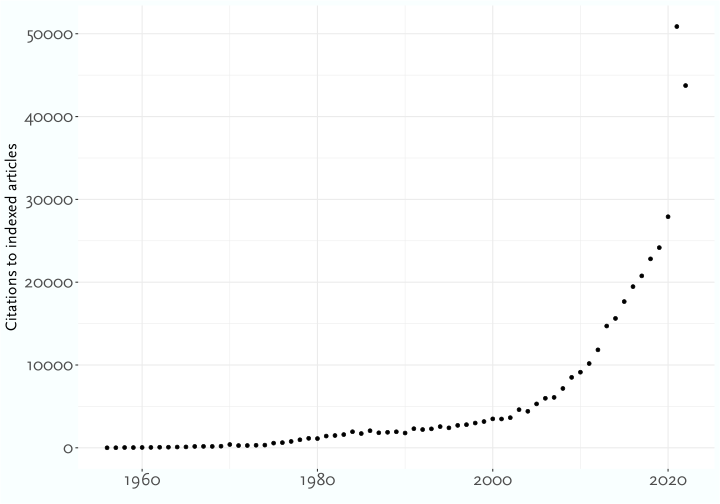
\includegraphics[keepaspectratio]{apc-2025-october-draft_files/figure-pdf/fig-citationsperyear-1.pdf}}

}

\caption{\label{fig-citationsperyear}The number of citations in the
dataset made each year.}

\end{figure}%

As noted in Section~\ref{sec-methodology}, I used a slightly different
method to extract the citations from 2022 onwards. It's possible that
the drop between 2021 and 2022 is a consequence of that change. However
I don't think it is for two reasons. First, it's more likely that 2021
is just an outlier; it's a consequence largely of \emph{Synthese}
publishing 1,439 articles in 2021, then a relatively few 509 articles in
2022. Second, I applied the method I'm using for 2022-2024 to 2020 and
2021, and got a fairly close agreement (within 1-2\%) with each year.

What explains this dramatic growth, at least through 2021? Part of the
explanation is that more articles are being published, and more articles
are being indexed. Figure~\ref{fig-articlesperyear} shows how many
articles are in the dataset each year.

\begin{figure}

\centering{

\pandocbounded{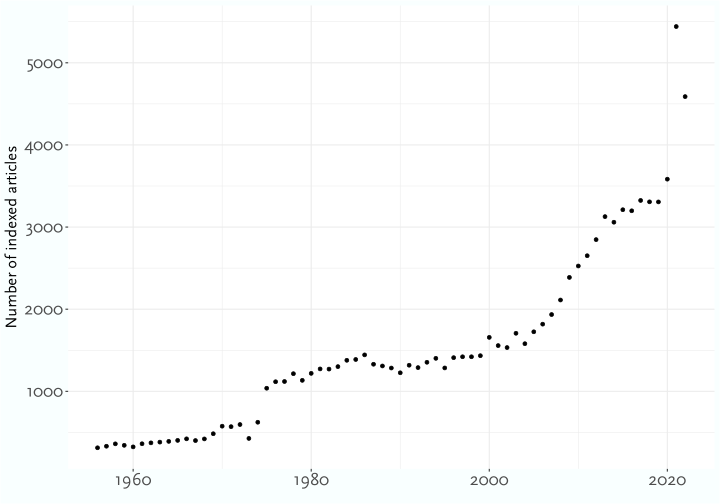
\includegraphics[keepaspectratio]{apc-2025-october-draft_files/figure-pdf/fig-articlesperyear-1.pdf}}

}

\caption{\label{fig-articlesperyear}The number of articles in the
dataset published each year.}

\end{figure}%

That explains some of the growth, but not all of it. The curve in
Figure~\ref{fig-articlesperyear} is not nearly as steep as the curve in
Figure~\ref{fig-citationsperyear}. The number of (indexed) citations per
article is also rising. In Figure~\ref{fig-outboundcitations} I've
plotted the average number of citations to other articles in the dataset
each year.

\begin{figure}

\centering{

\pandocbounded{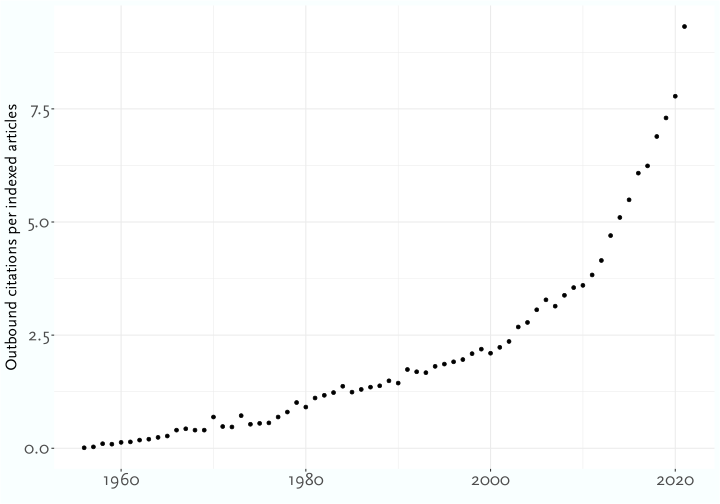
\includegraphics[keepaspectratio]{apc-2025-october-draft_files/figure-pdf/fig-outboundcitations-1.pdf}}

}

\caption{\label{fig-outboundcitations}The average number of citations to
indexed articles each year.}

\end{figure}%

There are a few possible explanations for the shape of this graph.

At the left-hand edge, there are obvious boundary effects. Since we're
only counting citations to articles published since 1956, it isn't
surprising that there aren't very many of them per article in the 1950s.
Since articles rarely get unpublished, there are more articles available
to cite every year.

That can't explain the massive jumps we see at the right hand edge of
Figure~\ref{fig-outboundcitations}. The jump there looks like the
convergence of two cultural trends. One is a trend simply to greater
numbers of citations. The most casual perusal of journals will confirm
that trend. The other is a trend to greater citations of journals
themselves, as opposed to books or edited volumes.

A sharp jump like this is a warning sign that there is something wrong
with the data, and so the data should be checked. It's impractical to
cross-check every entry, but those I have checked look correct. The
change seems led by the most prestigious journals. For each journal I
calculated the average number of outbound citations (to these hundred
journal) for both the 2010s, and the first two years of the 2020s. The
ten journals with the largest increase between the decades are shown in
Table~\ref{tbl-large-growth}.

\begin{longtable}[]{@{}
  >{\raggedright\arraybackslash}p{(\linewidth - 6\tabcolsep) * \real{0.5694}}
  >{\raggedleft\arraybackslash}p{(\linewidth - 6\tabcolsep) * \real{0.1389}}
  >{\raggedleft\arraybackslash}p{(\linewidth - 6\tabcolsep) * \real{0.1389}}
  >{\raggedleft\arraybackslash}p{(\linewidth - 6\tabcolsep) * \real{0.1528}}@{}}

\caption{\label{tbl-large-growth}Mean outbound citations for some
journals over the last two decades.}

\tabularnewline

\toprule\noalign{}
\begin{minipage}[b]{\linewidth}\raggedright
Journal
\end{minipage} & \begin{minipage}[b]{\linewidth}\raggedleft
2010-2019
\end{minipage} & \begin{minipage}[b]{\linewidth}\raggedleft
2020-2024
\end{minipage} & \begin{minipage}[b]{\linewidth}\raggedleft
Difference
\end{minipage} \\
\midrule\noalign{}
\endhead
\bottomrule\noalign{}
\endlastfoot
Philosophical Review & 14.8 & 26.3 & 11.5 \\
Philosophical Perspectives & 11.3 & 19.2 & 7.9 \\
Noûs & 11.5 & 18.4 & 6.9 \\
Philosophy and Phenomenological Research & 9.6 & 15.8 & 6.2 \\
Philosophical Studies & 9.0 & 14.6 & 5.6 \\
Journal of Philosophy & 9.0 & 14.5 & 5.6 \\
Philosophy & 4.0 & 8.9 & 4.9 \\
Episteme & 8.1 & 12.9 & 4.9 \\
Philosophical Quarterly & 8.8 & 13.6 & 4.7 \\
Philosophy Compass & 11.2 & 15.9 & 4.7 \\

\end{longtable}

Since \emph{Philosophical Review} only publishes 10 to 12 articles per
year, it is not surprising that it shows the most variation on this
list. Still, the change in the 2010s isn't only small sample size
variation. Of the 22 articles it published in 2020 and 2021, only one of
them \citep{WOS000575210400003} had fewer than 14.8 outbound citations.
With a sample of just 22 anything could happen, but it would be
surprising to have all but one end up on the same side of the historical
average by chance.

We could just ask what proportion of all citations accrue to an article
in a given year. But that would be an overcorrection. In the 2020s there
are more citations to be shared around, but also more articles to share
them between. We need to adjust for both things. Here's the way I'll do
it.

Say an article is from a year that is one of the \emph{typically} cited
articles iff it is between 3 and 10 years before the citing year. As we
saw in Figure~\ref{fig-master-citation-ratio}, that is when citations
typically peak. Using this definition, Figure~\ref{fig-articlecounts}
shows how many of these typically cited articles there are at any given
time. (So for 2000, it shows the number of articles published
1990-1997.)

\begin{figure}

\centering{

\pandocbounded{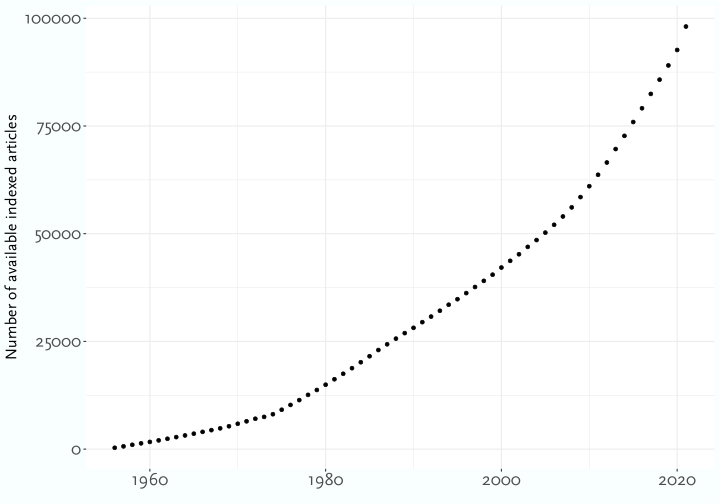
\includegraphics[keepaspectratio]{apc-2025-october-draft_files/figure-pdf/fig-articlecounts-1.pdf}}

}

\caption{\label{fig-articlecounts}Typically cited articles.}

\end{figure}%

In Figure~\ref{fig-citationcounts}, I've shown how often, in each year,
these `typical' articles are cited, and in Figure~\ref{fig-citationrate}
I've shown the mean number of citations to these typical articles there
are in each year.

\begin{figure}

\centering{

\pandocbounded{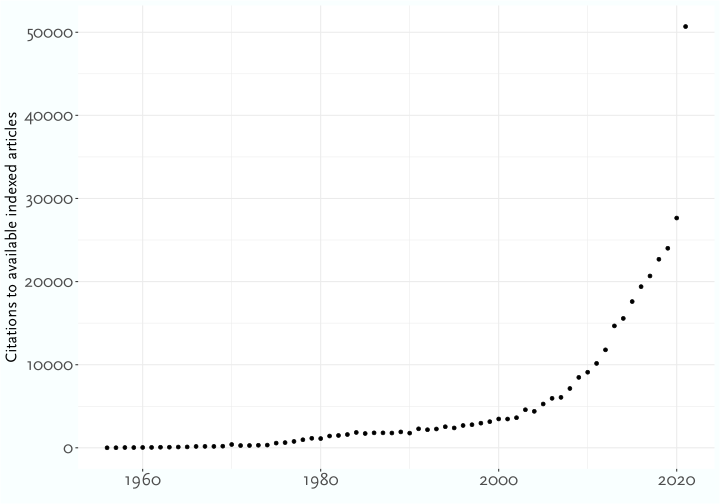
\includegraphics[keepaspectratio]{apc-2025-october-draft_files/figure-pdf/fig-citationcounts-1.pdf}}

}

\caption{\label{fig-citationcounts}Citations to typical articles.}

\end{figure}%

\begin{figure}

\centering{

\pandocbounded{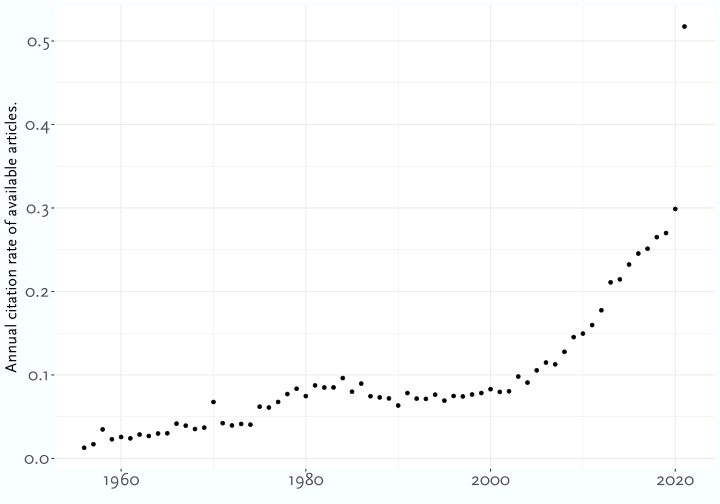
\includegraphics[keepaspectratio]{apc-2025-october-draft_files/figure-pdf/fig-citationrate-1.pdf}}

}

\caption{\label{fig-citationrate}Mean annual citations to typical
articles.}

\end{figure}%

Two things stand out about Figure~\ref{fig-citationrate}. The graph is
fairly flat for a long time. Between the mid 1970s and early 2000s it
bounces around without moving much. Then it takes off, and go through
the roof in 2021, before returning to the long term trend. The other
thing is that the numbers are never high. For most of this study, even
articles from this peak citation age, three to ten years old, are cited
in one of these hundred journals once a \emph{decade}. Actually, since
citation rates are extremely long-tailed, and mean rates are well above
medians, that somewhat overstates how often the `average article' was
being cited. Frequent citation is very much not the norm.\footnote{In
  the long run the average number of times an article is cited equals
  the average number of citations per article. So it shouldn't be too
  surprising that most article have just a handful of citations in
  philosophy journals.}

My first pass measure of an article's influence at a time is how often
it is cited at that time, divided by how often the typical article is
cited at that time. This is a little arbitrary; I could have picked
other ranges than three to ten years, but I think it gets things roughly
right. I tried several other measures, and they all either led to
implausible trends in the data, or to comparative judgments about the
influence of various papers that didn't seem remotely plausible. This
measure had the nice consequence that how influential the leading 50
articles from a period were 10-20 years after that period was reasonably
stable, suggesting that it does correct for period effects reasonably
well.

\section{Age Effects}\label{sec-age}

The next task is to work out how the age of an article affects how often
it is cited. The simplest thing to do here would be to look at a typical
year, and see how often articles from that year have been cited over
time. That would, unfortunately, be completely wrong.
Figure~\ref{fig-1990-outbound-citations} shows how often articles from
1990 have been cited over time.

\begin{figure}

\centering{

\pandocbounded{\includegraphics[keepaspectratio]{apc-2025-october-draft_files/figure-pdf/fig-1990-outbound-citations-1.pdf}}

}

\caption{\label{fig-1990-outbound-citations}Citations to articles
published in 1990.}

\end{figure}%

If we're using citations as a measure of influence,
Figure~\ref{fig-1990-outbound-citations} suggests that, collectively,
articles from 1990 were most influential in 2021. That's not really
true; they were most influential two to four years after they were
published, like most articles. It's just that there are so many articles
published in the 2020s, and each of them cite so many pieces, that
citations to three decade old articles get lifted by the rising tide.

A more intuitive way of measuring influence uses the notion of typical
articles from the Section~\ref{sec-period}. Let's adjust
Figure~\ref{fig-1990-outbound-citations} by dividing each value by two
things. First, by the citation rate of typical articles, as shown in
Figure~\ref{fig-citationrate}, to adjust for period effects. Second, by
the number of articles published in 1990, so we're getting a measure of
influence per article. The result what I earlier called the citation
ratio, and the graph for 1990's citation ratio is
Figure~\ref{fig-1990-outbound-citations-norm}.

\begin{figure}

\centering{

\pandocbounded{\includegraphics[keepaspectratio]{apc-2025-october-draft_files/figure-pdf/fig-1990-outbound-citations-norm-1.pdf}}

}

\caption{\label{fig-1990-outbound-citations-norm}Normalised measure of
citations to articles published in 1990.}

\end{figure}%

There are two reasons to think that the graph in
Figure~\ref{fig-1990-outbound-citations-norm} is a more plausible
measure of influence than the one in
Figure~\ref{fig-1990-outbound-citations}. One is just an appeal to
intuition. I know how often work from 1990 came up in discussions in the
1990s and in the 2020s, and it was a lot higher in the former than in
the latter. While that kind of intuitive evidence should be given some
weight, it's obviously unreliable on its own. The better reason is that
we get a very similar shaped graph to
Figure~\ref{fig-1990-outbound-citations-norm} no matter which initial
year we pick. This was already visible in
Figure~\ref{fig-decades-cite-ratio}, but it's worth seeing how stable it
is.

I've used the expression `citation ratio' a few times; it's worth being
more precise about what it is. Let \emph{c}(\emph{o},~\emph{n}) be the
number of citations of articles from year \emph{o} (the old year) in
year \emph{n} (the new year). Let \emph{a}(\emph{o}) be the number of
articles published in year \emph{o}. Then the citation ratio
\emph{r}(\emph{o}, \emph{n}) is:

\[
r(o, n) = \left(\frac{c(o, n)}{a(o)}\right) / \left(\frac{\sum\limits_{i = n-10}^{n-3}c(i, n)}{\sum\limits_{i = n-10}^{n-3}a(i)}\right)
\]

In Figure~\ref{fig-ageeffecttibble-early} and
Figure~\ref{fig-ageeffecttibble-late} each facet is a different value
for \emph{o}, the x-axis is \emph{n}, and the \emph{y} axis is
\emph{r}(\emph{o}, \emph{n}). The key thing to note is how steady these
graphs are. I have cheated a little; if I'd shown earlier years the
shapes would not have been the same. There are so few citations in the
1960s that the noise overwhelms the signal. Since then, we get a
reasonably steady pattern.

\begin{figure}

\centering{

\pandocbounded{\includegraphics[keepaspectratio]{apc-2025-october-draft_files/figure-pdf/fig-ageeffecttibble-early-1.pdf}}

}

\caption{\label{fig-ageeffecttibble-early}Citation rates for articles
published 1968-1992.}

\end{figure}%

\begin{figure}

\centering{

\pandocbounded{\includegraphics[keepaspectratio]{apc-2025-october-draft_files/figure-pdf/fig-ageeffecttibble-late-1.pdf}}

}

\caption{\label{fig-ageeffecttibble-late}Citation rates for articles
published 1993-2017.}

\end{figure}%

\section{Appendix: Summary Statistics}\label{sec-statistics}

The paper uses the journals shown in Table~\ref{tbl-list-of-journals}.

\begin{longtable}[]{@{}
  >{\raggedright\arraybackslash}p{(\linewidth - 10\tabcolsep) * \real{0.4274}}
  >{\raggedleft\arraybackslash}p{(\linewidth - 10\tabcolsep) * \real{0.0940}}
  >{\raggedleft\arraybackslash}p{(\linewidth - 10\tabcolsep) * \real{0.0855}}
  >{\raggedleft\arraybackslash}p{(\linewidth - 10\tabcolsep) * \real{0.0769}}
  >{\raggedleft\arraybackslash}p{(\linewidth - 10\tabcolsep) * \real{0.1624}}
  >{\raggedleft\arraybackslash}p{(\linewidth - 10\tabcolsep) * \real{0.1538}}@{}}

\caption{\label{tbl-list-of-journals}Journals used in this paper}

\tabularnewline

\toprule\noalign{}
\begin{minipage}[b]{\linewidth}\raggedright
Journal
\end{minipage} & \begin{minipage}[b]{\linewidth}\raggedleft
First Year
\end{minipage} & \begin{minipage}[b]{\linewidth}\raggedleft
Last Year
\end{minipage} & \begin{minipage}[b]{\linewidth}\raggedleft
Articles
\end{minipage} & \begin{minipage}[b]{\linewidth}\raggedleft
Outbound Citations
\end{minipage} & \begin{minipage}[b]{\linewidth}\raggedleft
Inbound Citations
\end{minipage} \\
\midrule\noalign{}
\endhead
\bottomrule\noalign{}
\endlastfoot
American Philosophical Quarterly & 1964 & 2024 & 1835 & 7759 & 10295 \\
Analysis & 1975 & 2024 & 2719 & 7494 & 14833 \\
Analytic Philosophy & 2016 & 2024 & 190 & 2218 & 501 \\
Archiv für Geschichte der Philosophie & 1975 & 2024 & 672 & 1598 &
1019 \\
Australasian Journal of Philosophy & 1975 & 2024 & 1736 & 10463 &
13439 \\
Biology and Philosophy & 1988 & 2024 & 1225 & 6179 & 4825 \\
British Journal for the History of Philosophy & 2007 & 2024 & 834 & 2465
& 1113 \\
British Journal for the Philosophy of Science & 1956 & 2024 & 1620 &
9330 & 13032 \\
British Journal of Aesthetics & 1975 & 2024 & 1436 & 3556 & 3614 \\
Bulletin of Symbolic Logic & 1997 & 2024 & 443 & 1326 & 1139 \\
Canadian Journal of Philosophy & 1975 & 2023 & 1552 & 7772 & 5732 \\
Croatian Journal of Philosophy & 2007 & 2024 & 376 & 1901 & 299 \\
Dialogue & 1975 & 2024 & 1555 & 3697 & 1105 \\
Economics and Philosophy & 1986 & 2024 & 568 & 2607 & 2386 \\
Episteme & 2005 & 2024 & 586 & 5196 & 3127 \\
Ergo & 2016 & 2024 & 386 & 5090 & 867 \\
Erkenntnis & 2000 & 2024 & 1780 & 17201 & 7630 \\
Ethical Theory and Moral Practice & 2008 & 2024 & 902 & 5874 & 2153 \\
Ethics & 1956 & 2024 & 1647 & 5758 & 15681 \\
Ethics and Information Technology & 2001 & 2024 & 567 & 1953 & 1032 \\
European Journal for Philosophy of Science & 2011 & 2024 & 562 & 5952 &
1473 \\
European Journal of Philosophy & 1998 & 2024 & 994 & 5839 & 3023 \\
Heythrop Journal & 1975 & 2024 & 1559 & 874 & 355 \\
History and Philosophy of Logic & 1992 & 2024 & 522 & 1447 & 930 \\
Hypatia & 2009 & 2024 & 683 & 1556 & 1711 \\
Inquiry & 1966 & 2024 & 1646 & 7186 & 4545 \\
International Journal for Philosophy of Religion & 1975 & 2024 & 1149 &
2183 & 1135 \\
International Philosophical Quarterly & 1961 & 2023 & 1588 & 1464 &
713 \\
Journal of Aesthetics and Art Criticism & 1975 & 2024 & 1539 & 3747 &
3757 \\
Journal of Applied Philosophy & 2006 & 2024 & 666 & 3473 & 1303 \\
Journal of Chinese Philosophy & 1973 & 2024 & 1278 & 1053 & 964 \\
Journal of Consciousness Studies & 2000 & 2024 & 1525 & 4939 & 3659 \\
Journal of Indian Philosophy & 1975 & 2024 & 1107 & 1477 & 1473 \\
Journal of Medical Ethics & 1975 & 2024 & 4340 & 5875 & 5091 \\
Journal of Moral Philosophy & 2005 & 2024 & 392 & 2449 & 979 \\
Journal of Philosophical Logic & 1972 & 2024 & 1497 & 7755 & 9811 \\
Journal of Philosophical Research & 2005 & 2024 & 463 & 2097 & 573 \\
Journal of Philosophy & 1956 & 2024 & 2761 & 7299 & 37873 \\
Journal of Political Philosophy & 1998 & 2023 & 609 & 2303 & 2886 \\
Journal of Social Philosophy & 2008 & 2024 & 508 & 2202 & 883 \\
Journal of Symbolic Logic & 1966 & 2024 & 4363 & 6757 & 10587 \\
Journal of Value Inquiry & 1980 & 2024 & 1369 & 2974 & 1466 \\
Journal of the American Philosophical Association & 2015 & 2024 & 340 &
2764 & 938 \\
Journal of the History of Ideas & 1956 & 2024 & 2212 & 995 & 1705 \\
Journal of the History of Philosophy & 1975 & 2024 & 1138 & 2800 &
3065 \\
Journal of the Philosophy of History & 2010 & 2024 & 284 & 618 & 187 \\
Kant-Studien & 1975 & 2024 & 1134 & 1708 & 1709 \\
Kantian Review & 2010 & 2024 & 337 & 1557 & 649 \\
Kennedy Institute of Ethics Journal & 1995 & 2024 & 574 & 1234 & 931 \\
Law and Philosophy & 1982 & 2024 & 852 & 2566 & 1518 \\
Linguistics and Philosophy & 1979 & 2024 & 878 & 5014 & 6408 \\
Logique et Analyse & 2007 & 2021 & 340 & 1565 & 336 \\
Metaphilosophy & 1975 & 2024 & 1562 & 4541 & 2837 \\
Mind & 1956 & 2024 & 1980 & 8454 & 18442 \\
Mind \& Language & 1994 & 2024 & 893 & 5807 & 6363 \\
Minds and Machines & 1992 & 2024 & 756 & 3442 & 1963 \\
Monist & 1963 & 2024 & 1975 & 4322 & 6444 \\
Notre Dame Journal of Formal Logic & 2009 & 2024 & 486 & 1661 & 707 \\
Noûs & 1975 & 2024 & 1480 & 11791 & 20557 \\
Pacific Philosophical Quarterly & 1980 & 2024 & 1231 & 7609 & 6542 \\
Philosophers' Imprint & 2010 & 2024 & 402 & 5177 & 3301 \\
Philosophia & 1975 & 2024 & 2249 & 10028 & 2917 \\
Philosophia Mathematica & 2008 & 2024 & 243 & 1613 & 897 \\
Philosophical Explorations & 2008 & 2024 & 390 & 2857 & 1271 \\
Philosophical Forum & 1971 & 2024 & 851 & 1726 & 612 \\
Philosophical Investigations & 1983 & 2024 & 708 & 1057 & 588 \\
Philosophical Papers & 2009 & 2023 & 234 & 1379 & 444 \\
Philosophical Perspectives & 2007 & 2023 & 305 & 3380 & 3491 \\
Philosophical Psychology & 1991 & 2024 & 1312 & 7178 & 4225 \\
Philosophical Quarterly & 1975 & 2024 & 1450 & 8660 & 10722 \\
Philosophical Review & 1956 & 2024 & 1033 & 5214 & 25881 \\
Philosophical Studies & 1956 & 2024 & 5485 & 35126 & 38208 \\
Philosophy & 1956 & 2024 & 1811 & 2452 & 3609 \\
Philosophy \& Public Affairs & 1971 & 2024 & 733 & 2591 & 11768 \\
Philosophy Compass & 2015 & 2024 & 651 & 7939 & 1750 \\
Philosophy East and West & 1966 & 2024 & 1604 & 1980 & 1755 \\
Philosophy and Phenomenological Research & 1956 & 2024 & 3273 & 15150 &
21527 \\
Philosophy and Rhetoric & 1975 & 2024 & 927 & 1170 & 893 \\
Philosophy of Science & 1956 & 2024 & 3259 & 12888 & 24991 \\
Philosophy of the Social Sciences & 1975 & 2024 & 997 & 2550 & 1705 \\
Phronesis & 1975 & 2024 & 783 & 1227 & 1620 \\
Politics, Philosophy and Economics & 2008 & 2024 & 325 & 2025 & 779 \\
Ratio & 1974 & 2024 & 1090 & 3699 & 3603 \\
Res Philosophica & 2013 & 2024 & 360 & 2176 & 737 \\
Review of Metaphysics & 1956 & 2024 & 1616 & 1499 & 2434 \\
Review of Symbolic Logic & 2008 & 2024 & 578 & 3906 & 2721 \\
Russell & 1981 & 2024 & 345 & 427 & 303 \\
Social Epistemology & 2011 & 2024 & 489 & 2381 & 1034 \\
Social Philosophy and Policy & 1983 & 2024 & 973 & 2108 & 2550 \\
South African Journal of Philosophy & 1987 & 2024 & 793 & 1867 & 650 \\
Southern Journal of Philosophy & 1976 & 2024 & 1984 & 5194 & 3057 \\
Studia Logica & 2010 & 2024 & 734 & 2418 & 1007 \\
Studies in History and Philosophy of Science & 1974 & 2024 & 1832 & 8892
& 6217 \\
Synthese & 1966 & 2024 & 7770 & 64828 & 32888 \\
Theoria & 2007 & 2024 & 459 & 3902 & 723 \\
Theory and Decision & 1970 & 2024 & 1936 & 2101 & 2280 \\
Thought & 2016 & 2022 & 219 & 1537 & 455 \\
Topoi & 1982 & 2024 & 1327 & 5554 & 2363 \\
Transactions of the Charles S. Peirce Society & 1975 & 2024 & 1176 &
1874 & 1560 \\
Utilitas & 2009 & 2024 & 391 & 2480 & 1147 \\

\end{longtable}

What I've called an \emph{article} here is anything that either (a)
marked as an article or research-article by WoS, or (b) marked as a
review, discussion, or note by WoS and is at least 15 pages long. I
needed to include (b) because some very important works (e.g.,
\citet{WOSA1963CEU0700001} and \citet{WOS000272855000002}) were not
recorded as articles by WoS.

The years here are \textbf{not} the first and last years that the
journals published, but the earliest and latest years that are in the
WoS index (as of the time I pulled the data). As mentioned in the main
text, this makes a big difference for some journals, especially
\emph{Analysis}.

The way WoS handles the `supplements' to \emph{Noûs}, i.e.,
\emph{Philosophical Perspectives} and \emph{Philosophical Issues}, is a
little uneven. Some years these are recorded as being their own thing,
i.e., with a source name of \emph{Philosophical Perspectives} or
\emph{Philosophical Issues}; and some years they are recorded as special
issues of \emph{Noûs}. When they were listed as special issues, the
citations were extremely unreliable. Some high profile articles are
recorded as having no citations until several years after publication.
The bibliographic information for the articles themselves was also
spotty. So I've manually removed all records that were listed as special
or supplementary issues of \emph{Noûs} (and similarly removed the
citations to those articles that did get tracked). What you see here are
just the standalone issues of \emph{Philosophical Perspectives}.


\bibliography{/Users/weath/Documents/quarto-articles/brian-quarto.bib,/Users/weath/Documents/citations-2025/autobib.bib}



\end{document}
